\section{Verteilte Systeme}

\section*{11 Vorlesung 11}
\subsection*{11.1 Verteiltes System Definition + Einsatz}
Ein verteiltes System besteht aus einer Sammlung autonomer Computer (Knoten) und Softwarebausteinen (Komponenten), die über ein Netzwerk miteinander verbunden sind und gemeinsam als ein einziges System arbeiten. Sie werden in verschiedenen Bereichen eingesetzt, darunter Datenbanken, CloudComputing, verteilte Anwendungen usw.

\begin{itemize}
  \item Oft sehr gross
  \item Sehr datenorientiert: Datenbanken im Zentrum der Anwendung
  \item Extrem interaktiv: GUI, aber auch Batch
  \item Sehr nebenläufig: Grosse Anzahl an parallel arbeitenden Benutzern
  \item Oft hohe Konsistenzanforderungen
\end{itemize}

\subsection*{11.2 Verteiltes System Konzepte + Architekturstil}
Verteilte Systeme basieren auf verschiedenen Konzepten und Architekturstilen:

\subsection*{11.2.1 Kommunikationsverfahren}
Kommunikationsverfahren umfassen Methoden, mit denen die einzelnen Knoten in einem verteilten System miteinander kommunizieren können. Dazu gehören beispielsweise Remote Procedure Calls (RPC), Message Queuing und Publish-Subscribe-Systeme.

\subsection*{11.2.2 Fehlertoleranz}
Fehlertoleranz ist ein wichtiger Aspekt verteilter Systeme, der sicherstellt, dass das System auch bei Ausfällen oder Fehlern in einzelnen Komponenten weiterhin zuverlässig arbeitet. Hierzu werden Mechanismen wie Replikation, Failover und Fehlererkennung eingesetzt.

\subsection*{11.2.3 Fehlersemantik}
Die Fehlersemantik beschreibt das Verhalten eines verteilten Systems im Falle von Fehlern oder Ausfällen. Dies umfasst Aspekte wie Konsistenzgarantien, Recovery-Verfahren und Kompensationsmechanismen.

\subsection*{11.3 Design- und Implementierungsaspekte von Client-ServerSystemen}
Client-Server-Systeme sind eine häufige Architektur für verteilte Systeme, bei der Clients Anfragen an einen zentralen Server senden, der diese verarbeitet und entsprechende Antworten zurückgibt. Design- und Implementierungsaspekte umfassen unter anderem die Aufteilung von Funktionalitäten zwischen Client und Server, die Wahl der Kommunikationsprotokolle und die Skalierbarkeit des Systems.

\subsection*{11.4 Verteiltes System Architektur + Design Patterns}
Die Architektur verteilter Systeme kann durch verschiedene Design Patterns strukturiert werden, um wiederkehrende Probleme effizient zu lösen. Dazu gehören Patterns wie Master-Slave, Peer-to-Peer, Publish-Subscribe, sowie verschiedene Replikations- und Verteilungsstrategien.\\
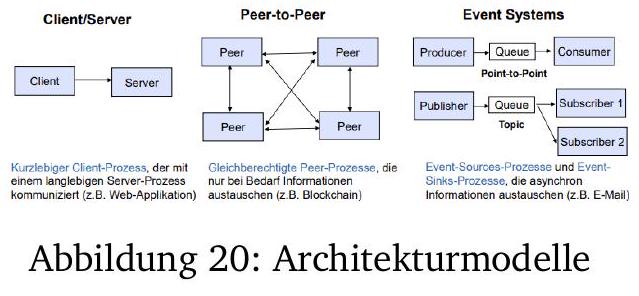
\includegraphics[width=\linewidth]{images/2024_12_29_0d1d7b5551ea1b4b41bdg-18}

\subsection*{11.5 Gängige Technologien (Middleware) f. Informationssysteme und Internet-basierte Systeme}
Für die Entwicklung verteilter Systeme stehen verschiedene MiddlewareTechnologien zur Verfügung, die die Kommunikation und Integration von verteilten Komponenten erleichtern. Dazu gehören Messaging-Broker wie Apache

Kafka, Middleware-Frameworks wie CORBA (Common Object Request Broker Architecture) und RESTful Web Services.

